\documentclass[12pt]{article}
\usepackage{polski}
\usepackage[utf8]{inputenc}
\usepackage{fullpage}
\usepackage{tabto}
\usepackage{graphicx} 
\usepackage{float}
\usepackage{caption}
\usepackage{indentfirst} 

%zmienić napis rysunek na tabela w tabelach
%dodać ref-y
%dodać srakowatą table bezpośrednio po 5.Wynki
%dodać "z normalizacją"
%dodac bibliografie do rysunkow

\linespread{1.3}
\begin{document}
%---------------------------------------------------------
%					Strona Tytułowa
%---------------------------------------------------------
\begin{titlepage}
%-----------------------Tytuł-----------------------------
\newcommand{\LINE}{\rule{\linewidth}{0.7mm}}
\center
\LINE \\[0.5cm]
\Large\textsc{Komputerowe wspomaganie diagnozowania nowotworów piersi z wykorzystaniem algorytmów minimalno-odległościowych}\\ [5mm]
\normalsize\textsc{Zastosowanie Informatyki w Medycynie}  \\[0.5cm]
\LINE \\[3cm]
%----------------------Nazwiska---------------------------
\begin{minipage}{0.5\textwidth}
\begin{flushleft} \large
\emph{Autorzy:}
		\\Mateusz Ożóg %226125
		\\Grzegorz Milaszkiewicz %226110
\end{flushleft}
\end{minipage}
~
\begin{minipage}{0.45\textwidth}
\begin{flushright} \large
\emph{Prowadzący:} \\
mgr inż. Jakub Klikowski
\end{flushright}
\end{minipage}\\[2cm]
%----------------------Stopka-----------------------------
\vfill
\center Wrocław 2019
\end{titlepage}

%---------------------------------------------------------
%					Spis treści
%---------------------------------------------------------
\renewcommand{\contentsname}{Spis treści}
\tableofcontents
\newpage

%---------------------------------------------------------
%					Część pierwsza
%---------------------------------------------------------
\section{Charakterystyka analizowanego problemu}
Tematem naszego projektu jest wspomniane w tytule, komputerowe wspomaganie diagnozowania nowotworów piersi przy pomocy algorytmów minimalno-odległościowych. Na podstawie empirycznego materiału diagnostycznego należało zbadać poprawność diagnoz losowo wybranych pacjentów dla zaimplementowanych mechanizmów rozpoznawania.
\newline
\indent Pojedyncza diagnoza przyporządkowuje pacjentkę do jednej z wyodrębnionych klas. Przeprowadzana jest na podstawie pewnych cech przypisywanych do danego osobnika. Poszczególne klasy posiadają charakterystyczne wartości wyróżnionych parametrów. W procesie rozpoznawania każdy z parametrów pomaga określić przynależność do danej kategorii. Wartości niektórych z nich mogą jednoznacznie determinować klasę danego pacjenta, natomiast inne tylko ją zasugerować. W związku z tym zostały one posortowane malejąco, zgodnie z ich znaczeniem w procesie rozpoznawania. 
\newline \indent Dla ułatwienia zrozumienia problemu i dokonania jego dogłębnej analizy, poniżej przedstawimy krótką analizę danych poddawanych późniejszym badaniom.


\subsection{Analiza materiału diagnostycznego}
\indent Do badania przystąpiło 569 kobiet u ,których został zdiagnozowany rak piersi. Każda z nich została opisana za pomocą 33 wartości. Pierwszą jest numer identyfikacyjny. Druga składa się z dwóch liter M lub B i oznacza przynależność do danej klasy.  Grupa z rakiem łagodnym (357 kobiet) oznaczona jest literą B, natomiast z rakiem złośliwym (212 kobiet) literą M. Rozkład ilości pacjentów przynależnych do danych klas przedstawiony został na rysunku 1 (malignant - nowotwór złośliwy, benign - nowotwór łagodny). Pozostałe wartości wyznaczane były na podstawie wyglądu jądra komórkowego każdej z pacjentek.
\newline

\begin{figure}[H]
	\centering
		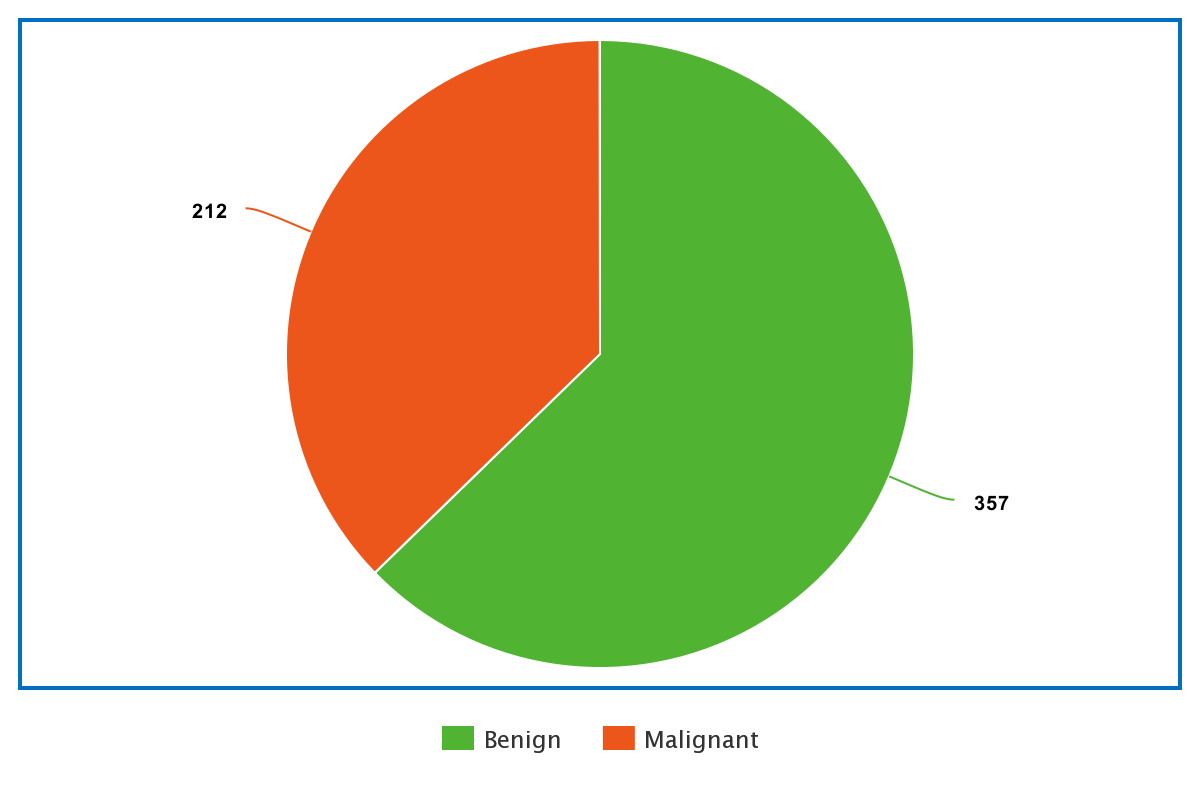
\includegraphics[scale=0.6]{images/pie_chart.png}
	\caption{Przynależność pacjentek do wyznaczonych klas}
\end{figure}

\indent U każdej z kobiet zostało wyróżnionych 10 cech głównych (tabela 2) oraz 20 dodatkowych opisujących błąd standardowy oraz najgorszą uzyskaną wartość dla każdej z nich. Razem wyznaczono 30 parametrów. 
\newline

\begin{table}[H]
\captionof{table}{Cechy jądra komórkowego wykorzystywane w procesie rozpoznawania} 

	\begin{tabular}{|p{0.2\linewidth}|p{0.74\linewidth}|}%{|l|l|}
	\hline\centering
	Numer cechy 	& Opis 				\\ \hline\centering
	1	& Promień (średnia odległość od środka do punktów na obwodzie) \\ \hline\centering
	2	& Tekstura (odchylenie standardowe wartości skali szarości) \\ \hline\centering
	3	& Obwód \\ \hline\centering
	4	& Powierzchnia \\ \hline\centering
	5	& Gładkość \\ \hline\centering
	6	& Ścisłość(obwód$^2/powierzchnia-1.0$) \\ \hline\centering
	7	& Wklęsłość (dotkliwość wklęsłych części konturu) \\ \hline\centering
	8	& Wklęsłe punkty (liczba wklęsłych części konturu) \\ \hline\centering
	9	& Symetria \\ \hline\centering
	10	& Wymiar fraktalny ("przybliżenie linii brzegowej" - 1) \\ \hline
	\end{tabular}
\end{table}
\indent Podsumowując analizę przedstawionego problemu rozpoznawania, pacjentów będziemy dzielić na dwie klasy. Więcej informacji empirycznej posiadamy na temat klasy reprezentującej nowotwór łagodny, co jest spowodowane większą liczbą kobiet w jego gronie. Każda z pacjentek posiada 30 cech, które przedstawione są za pomocą wielowartościowych liczb rzeczywistych. Pojedyncza cecha z pewną dokładnością wyznacza klasyfikację do danej klasy.W celu uzyskania dokładniejszych wyników w procesie rozpoznawania będziemy przeprowadzali ranking cech. Wykorzystuje on metody selekcji, które porządkują parametry pacjentów rozpoczynając od cech o największym znaczeniu. Sam proces rozpoznawania opierać się będzie na implementacji algorytmów minimalno-odległościowych tj. NM (nearest mean), KNN (k-nearest neighbours).

%---------------------------------------------------------
%					Część druga
%---------------------------------------------------------
\section{Opis stosowanych algorytmów}

\indent W procesie klasyfikacji pacjentów do poszczególnych klas zostaną wykorzystane algorytmy: najbliższej średniej oraz k-najbliższych sąsiadów. W przypadku drugiego algorytmu jako parametr k (ilość sąsiadów) zostaną przyjęte następujące wartości: 1, 5 oraz 9. Pacjentów będziemy dzielić na 2 grupy. Zbiór uczący będzie określał obiekty z zdiagnozowaną klasą. W zbiorze testowym natomiast będą znajdowali się pacjenci poddawani klasyfikacji na podstawie przetworzonych danych z grupy uczącej. Struktura danych w obu algorytmach jest identyczna. Każdy pacjent będzie określany za pomocą wektora cech tak jak to przedstawiono we wzorze poniżej.
\begin{center}
\[ x = (x_1, x_2, ... , x_n)\]
\end{center}


Każdy zbiór będzie składał się z m takich wektorów, gdzie m oznacza liczbę przypisanych do niego pacjentów.
Zbiór uczący i testujący będą wyglądały następująco:
\begin{center}
\[ (x_{11}, x_{12}, ... , x_{1n}), (x_{11}, ..., x_{12}, ... , x_{1n})\]
\end{center}

,gdzie w nawiasach okrągłych znajdują się dane poszczególnych pacjentów posiadających n cech, w naszym przypadku liczba ta wynosi 30.
\subsection{Algorytm najbliższej średniej}
\indent Algorytm polega na wyliczeniu obiektu centralnego (wykorzystując średnią arytmetyczną) dla każdej klasy. Jest on uśrednionym wektorem uwzględniającym wszystkie próbki ze zbioru uczącego należące do danej klasy. Na jego podstawie liczona będzie odległość do obiektu testowego, na którym przeprowadzana jest klasyfikacja. Obiekt ten opisany jest za pomocą poniższego wzoru.
\begin{center}
$ \sum{x}$
\end{center}
\begin{figure}[H]
	\centering
		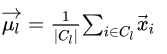
\includegraphics[scale=1]{images/nm_average.png}
	\caption{wzorek}
\end{figure}

Aby lepiej zobrazować działanie algorytmu przedstawiony zostanie prosty przykład bazujący na próbkach dających się umieścić w przestrzeni dwuwymiarowej. \newline
\begin{figure}[H]
	\centering
		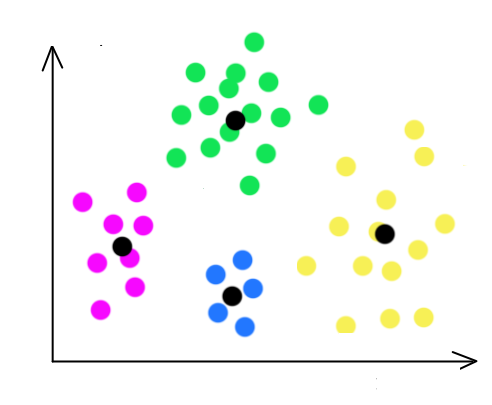
\includegraphics[scale=0.7]{images/nm_alg_example.png}
	\caption{Przykład działania algorytmu k najbliższych sąsiadów [1]}
\end{figure}

 
\indent Dla każdej klasy wyznaczany jest punkt średni, na podstawie którego dokonywana będzie klasyfikacja próbki testującej. 

\subsection{Algorytm k-najbliższych sąsiadów}
\indent Polega na znalezieniu k najbardziej podobnych próbek w zbiorze uczącym do obiektu testowego. Współczynnik k określa ilu sąsiadów będziemy szukać. Po ustaleniu sąsiedztwa sprawdzamy, z której klasy próbek jest najwięcej. Podobieństwo danych obiektów badane jest przy pomocy wybranych metryk odległościowych. Dla lepszego zobrazowania działania algorytmu, poniżej znajduje się prosty przykład bazujący na wektorach w przestrzeni dwuwymiarowej. \newline
\begin{figure}[H]
	\centering
		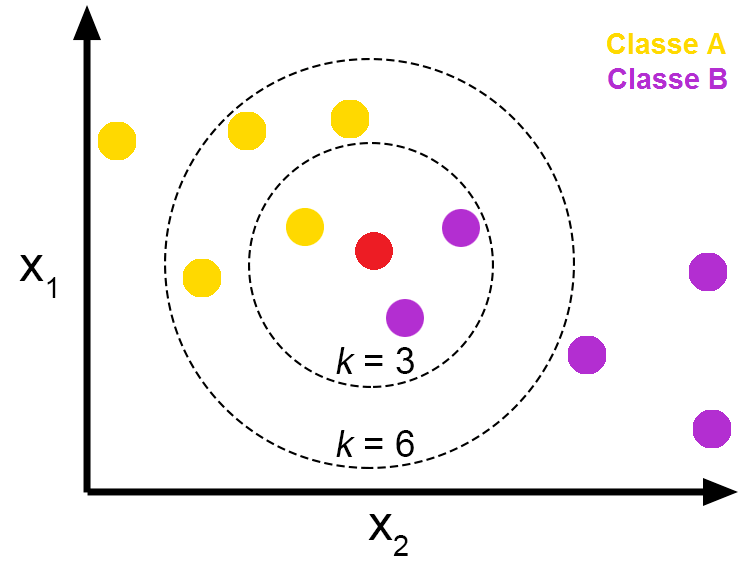
\includegraphics[scale=0.6]{images/knn_alg_example.png}
	\caption{Przykład działania algorytmu k najbliższych sąsiadów [1]}
\end{figure}

\indent Jak można zauważyć na przykładzie, klasyfikacja dla wartości parametru k równej 3 będzie przypisywała nasz obiekt testowy do klasy B, natomiast zwiększając wielkość sąsiędztwa sytuacja zmieni się.
%---------------------------------------------------------
%					Część Trzecia
%---------------------------------------------------------
\section{Informacja o środowisku implementacyjnym}

\indent Badania zostały przeprowadzone przy pomocy języka Python w wersji 3.6. Algorytmy zostały zaimplementowane z użyciem biblioteki sklearn wykorzystując metody KNeighborsClassifier oran NearestCentroid zwracające wybrany klasyfikator. Na jego podstawie trenowany był zbiór uczący przy pomocy metody fit, a następnie przy pomocy predict przyjmującej jako parametr zbiór testowy dokonywana była diagnoza. Otrzymane wartości klasyfikacji porównane były z rzeczywistym stanem badanego obiektu wykorzystując opisane w kolejnej części metryki klasyfikacji.


%---------------------------------------------------------
%					Część czwarta
%---------------------------------------------------------
\section{Opis badań eksperymentalnych}
\indent W badaniu zostały porównane algorytmy opisane w punkcie 2 niniejszej pracy. Dodatkowo każdy z nich został uruchomiony z różnymi parametrami wejściowymi tj. rodzaj metryki klasyfikacji, sposób mierzenia odległości pomiędzy próbkami, normalizacja wektora cech czy w przypadku algorytmu najbliższego sąsiada wielkość parametru k. Porównanie różnych wariantów tych wartości zostało umieszczone w kolejnym punkcie tej pracy. Poniżej przedstawiono szczegóły dotyczące przeprowadzonych badań.\\

\subsection{Parametry klasyfikacji}
W tabeli \ref{parametry_klasyfiacji} zostały przedstawione parametry klasyfikacji.
\begin{table}[H]
\captionof{table}{Parametry klasyfikacji} 
\label{parametry_klasyfiacji}
	\begin{tabular}{|p{0.3\linewidth}|p{0.64\linewidth}|}%{|l|l|}
	\hline\centering
	Rodzaj parametru 	& Testowane wartości 		\\ \hline\centering
	Metryki klasyfikacji	& accuracy, balanced, copen kappa \\ \hline\centering
	Algorytm	& NM, 1-NN, 5-NN, 9-NN \\ \hline\centering
	Metryka odległości	& euklides, manhatan \\ \hline\centering
	Wektor cech	& z normalizacją, bez normalizacji \\ \hline\centering
	Liczba cech	& Liczby naturalne z przedziału <1;30> \\ \hline
	\end{tabular}
\end{table}

Opis wykorzystanych metryk klasyfikacji:
\newline
accuracy - porównuje przewidywane wartości klasyfikacji z ich rzeczywistym stanem, diagnoza jest zgodna tylko w przypadku dokładnie przewidzianego wyniku.
\newline
balanced - metryka wykorzystywana przy niezbalansowanych zbiorach danych. Jest zdefiniowana jako średnia uzyskana dla każdej klasy [!].
\newline
copen kappa -  
\newline\newline
\indent Pozostałe parametry klasyfikacji zostały wyjaśnione we wcześniejszych rozważaniach pracy bądź zostały pominięte przez autorów pracy w związku z ich małym stopniem skomplikowania.
\newline
\indent  Przeprowadzenie badań odbyło się przy pomocy 5 razy powtarzanej metody 2-krotnej walidacji krzyżowej. Wszystkich pacjentów losowo podzieliliśmy na wspominany zbiór uczący oraz testujący. Następnie uruchamiamy na testowanych obiektach poszczególne algorytmy zmieniając kolejno wyżej wymienione rodzaje parametrów. Dodatkowo zmieniamy liczbę cech w wektorze opisującym próbki od wartości 1 aż do 30. Dla każdej konfiguracji zapisujemy wyniki. Po wykonanych badaniach zamieniamy zbiory. Zbiór uczący staje się testującym i na odwrót, zbiór testujący uczącym. Po raz kolejny wykonujemy badania a wyniki zapisujemy. Proces ten, rozpoczynający się od losowania zbioru powtarzamy pięciokrotnie, co sprawi, że osiągnięte wyniki będą pozbawione błędów grubych.
\newline
\indent W związku z dużą liczbą danych wynikających z liczbą zmiennych parametrów, badania nie są przeprowadzone dla wszystkich konfiguracji. Najpierw przeprowadzone zostało porównanie klasyfikatorów, biorąc pod uwagę wszystkie zaimplementowane algorytmy, wyznaczając najdokładniej działający. Następnie dla wybranego klasyfikatora przetestowano algorytmy, sprawdzając osiąganą przez nie dokładność. Dla najlepszej konfiguracji wspomnianych wyżej parametrów porównane zostały metryki odległości. Na koniec porównano wyniki osiągane z normalizacją wektora cech poszczególnych pacjentów oraz bez normalizacji. Osiągnięte rezultaty oraz wnioski z nich wynikające przedstawiono w dalszej części pracy.

%---------------------------------------------------------
%					Część piąta
%---------------------------------------------------------
\section{Wyniki}
\newpage 


% Porownanie metryk 

%-------------------------EUKLIDES--------------------------
\subsection{Porównanie metryk}
\subsubsection{Euklides}
\begin{figure}[H]
	\centering
		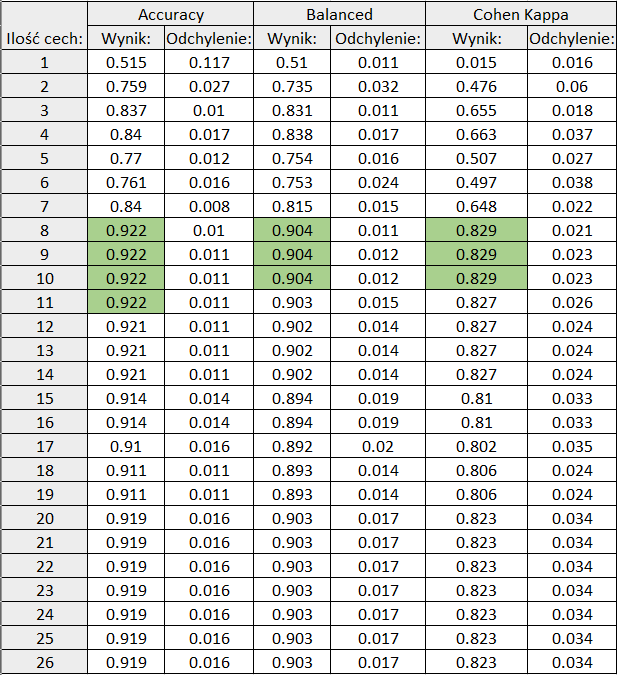
\includegraphics[scale=0.9]{images/metrics/9nn_euklides_norm_tab.png}
	\caption{Porównanie metryk dla algorytmu 9 najbliższych sąsiadów z normalizacją wektorów}
\end{figure}
\begin{figure}[H]
	\centering
		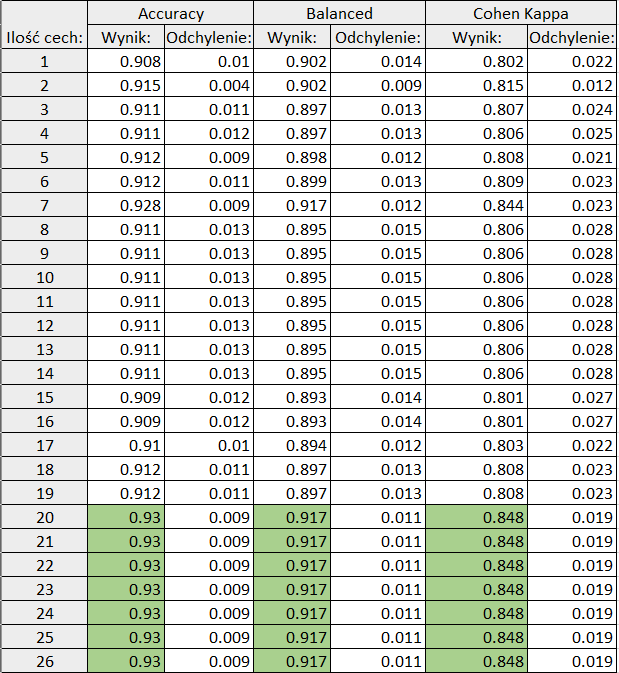
\includegraphics[scale=0.9]{images/metrics/9nn_euklides_beznorm_tab.png}
	\caption{Porównanie metryk dla algorytmu 9 najbliższych sąsiadów bez normalizacji wektorów}
\end{figure}

\begin{figure}[H]
	\centering
		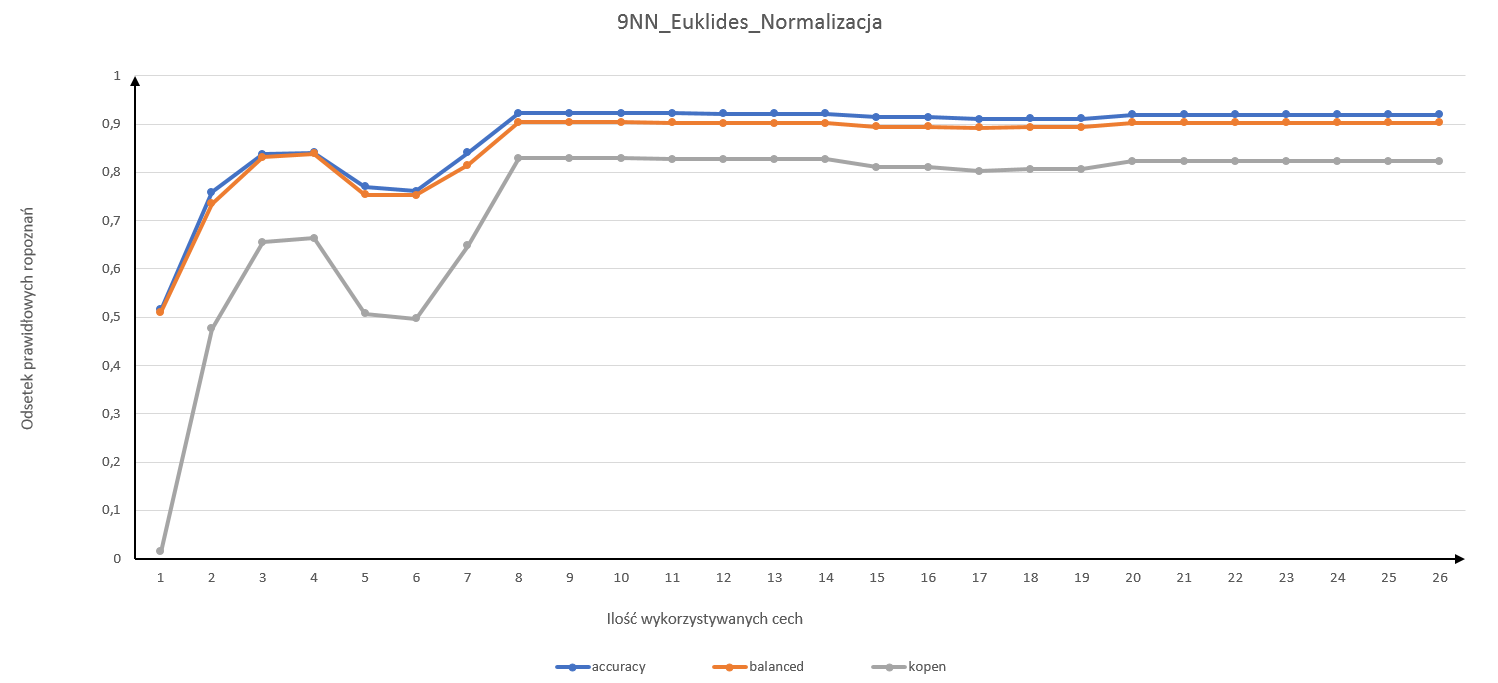
\includegraphics[scale=0.66]{images/metrics/9nn_euklides_norm.png}
	\caption{Porównanie metryk dla algorytmu 9 najbliższych sąsiadów z normalizacją wektorów}
\end{figure}
\begin{figure}[H]
	\centering
		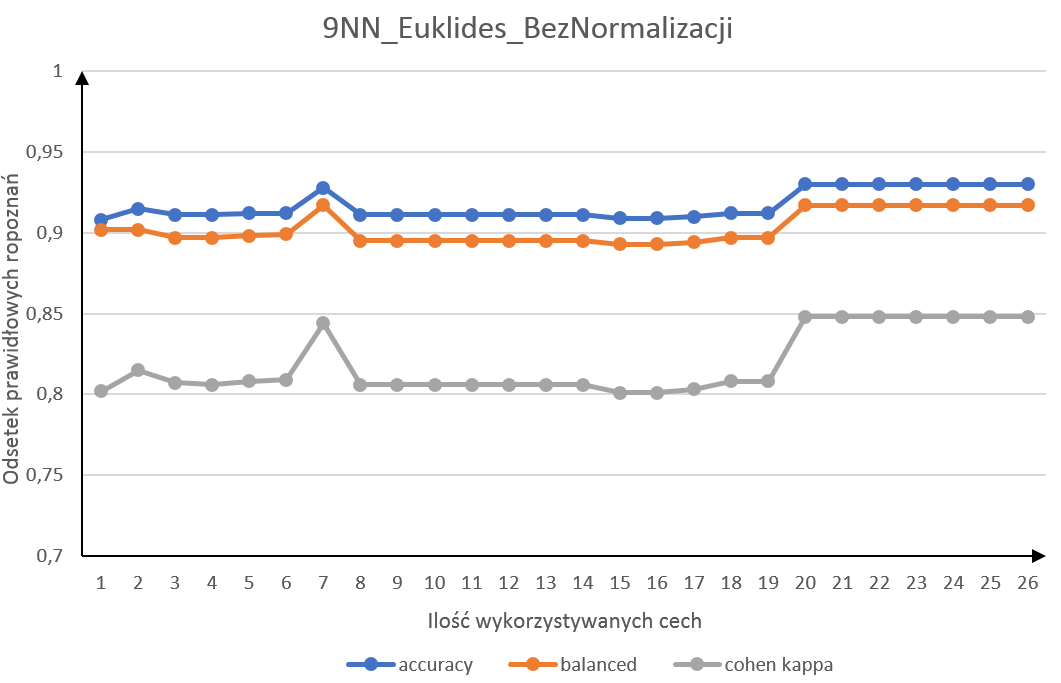
\includegraphics[scale=0.66]{images/metrics/9nn_euklides_beznorm.png}
	\caption{Porównanie metryk dla algorytmu 9 najbliższych sąsiadów bez normalizacji wektorów}
\end{figure}
%-------------------------EUKLIDES--------------------------

\subsubsection{Manhatan}
%-------------------------MANHATAN--------------------------
\begin{figure}[H]
	\centering
		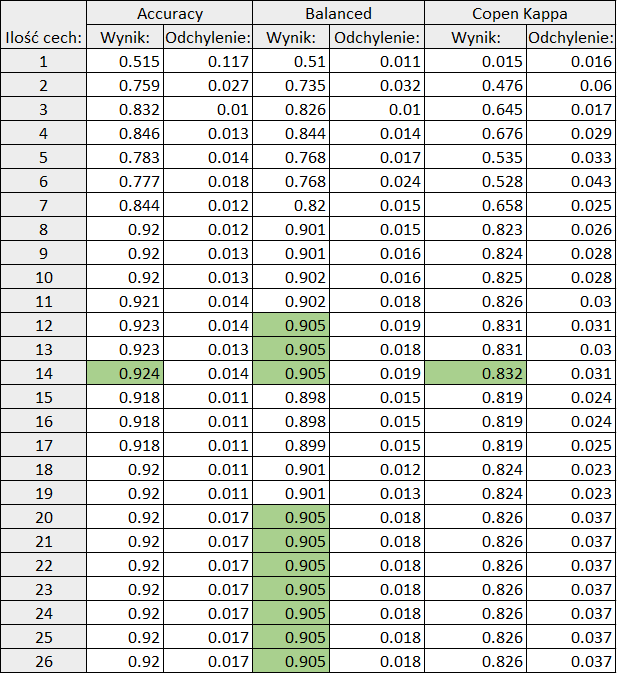
\includegraphics[scale=0.9]{images/metrics/9nn_manhatan_norm_tab.png}
	\caption{Porównanie metryk dla algorytmu 9 najbliższych sąsiadów z normalizacją wektorów}
\end{figure}
\begin{figure}[H]
	\centering
		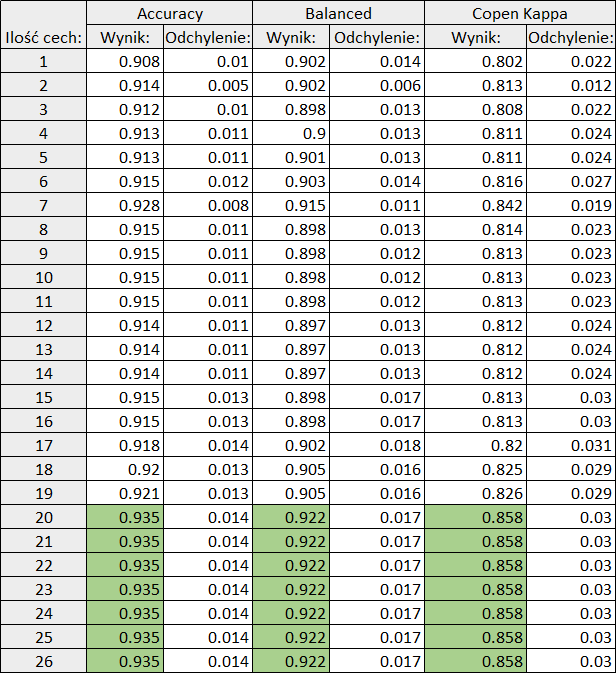
\includegraphics[scale=0.9]{images/metrics/9nn_manhatan_beznorm_tab.png}
	\caption{Porównanie metryk dla algorytmu 9 najbliższych sąsiadów bez normalizacji wektorów}
\end{figure}
\begin{figure}[H]
	\centering
		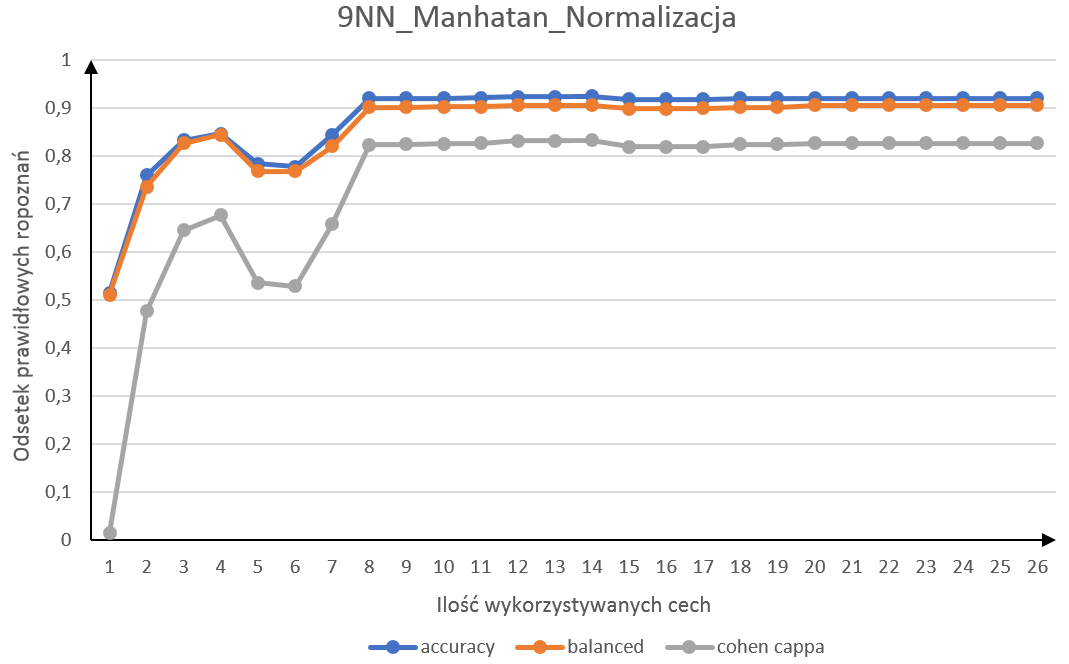
\includegraphics[scale=0.66]{images/metrics/9nn_manhatan_norm.png}
	\caption{Porównanie metryk dla algorytmu 9 najbliższych sąsiadów z normalizacją wektorów}
\end{figure}
\begin{figure}[H]
	\centering
		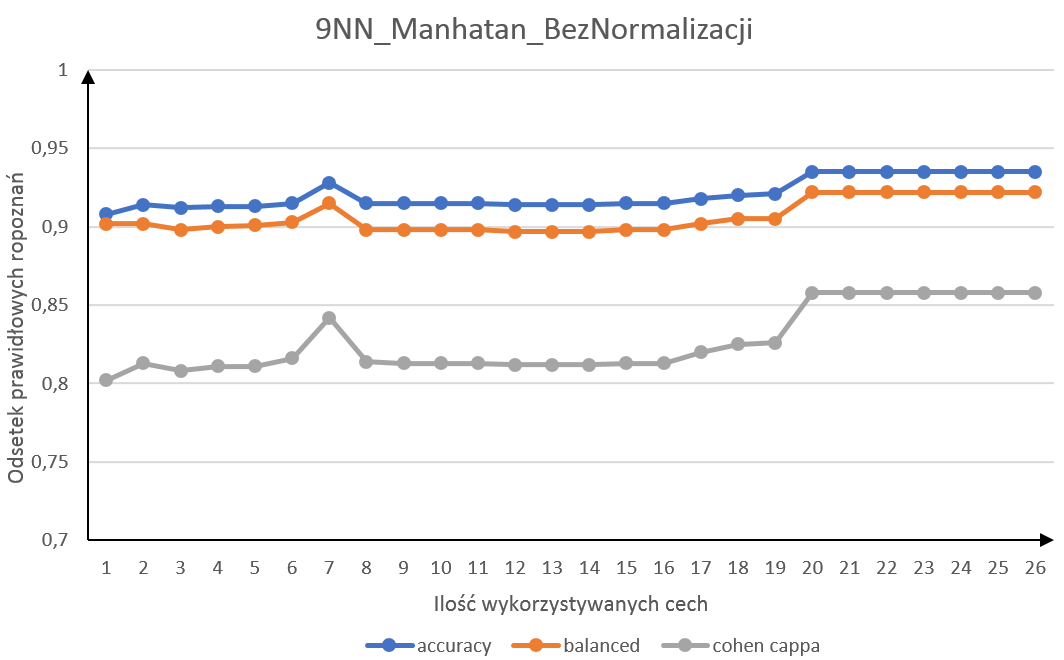
\includegraphics[scale=0.66]{images/metrics/9nn_manhatan_beznorm.png}
	\caption{Porównanie metryk dla algorytmu 9 najbliższych sąsiadów bez normalizacji wektorów}
\end{figure}
%-------------------------MANHATAN--------------------------
\subsection{Porównanie algorytmów}
%Porownanie algorytmów

\begin{figure}[H]
	\centering
		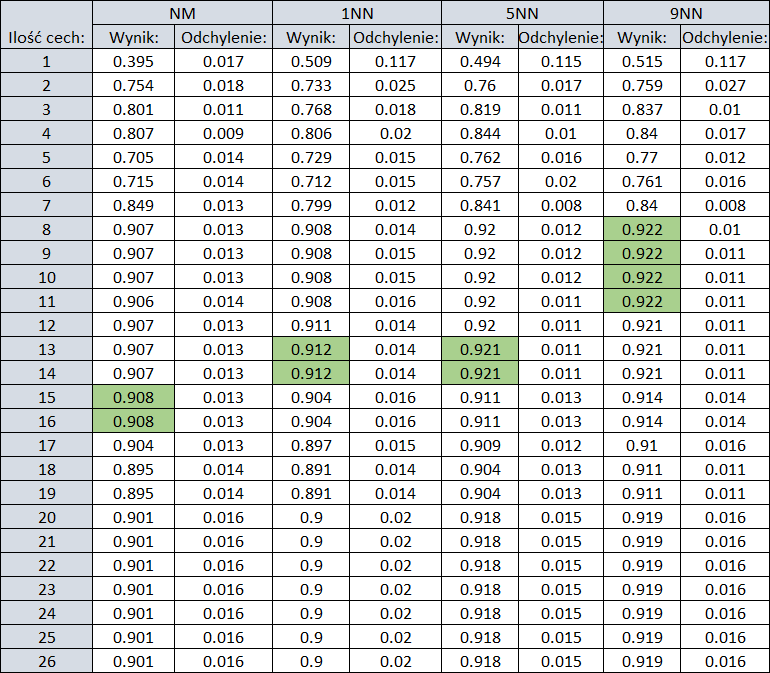
\includegraphics[scale=0.8]{images/algorithms/euklides_norm_tab.png}
	\caption{Porównanie algorytmów dla metryki odległościowej \textit{Euklides}}
\end{figure}

\begin{figure}[H]
	\centering
		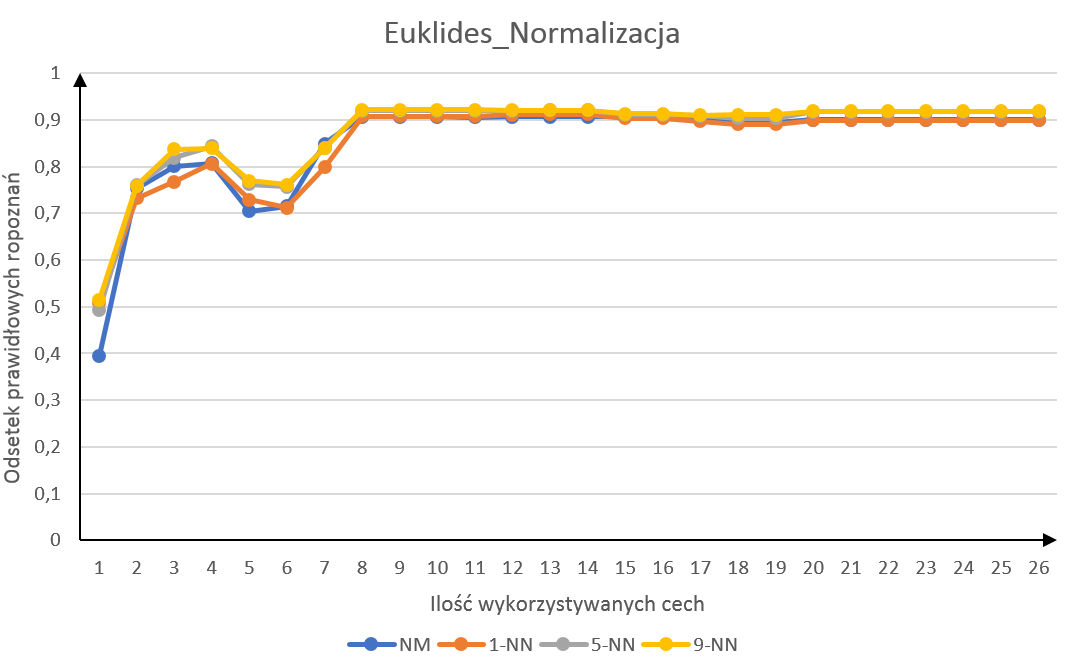
\includegraphics[scale=0.66]{images/algorithms/euklides_norm.png}
	\caption{Porównanie algorytmów dla metryki odległościowej \textit{Euklides}}
\end{figure}

\begin{figure}[H]
	\centering
		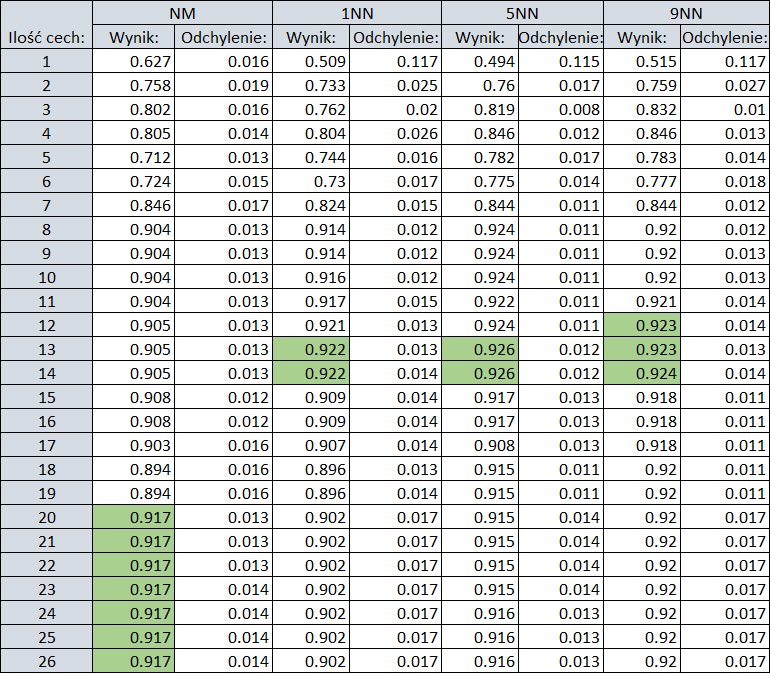
\includegraphics[scale=0.8]{images/algorithms/manhatan_norm_tab.png}
	\caption{Porównanie algorytmów dla metryki odległościowej \textit{Manhatan}}
\end{figure}

\begin{figure}[H]
	\centering
		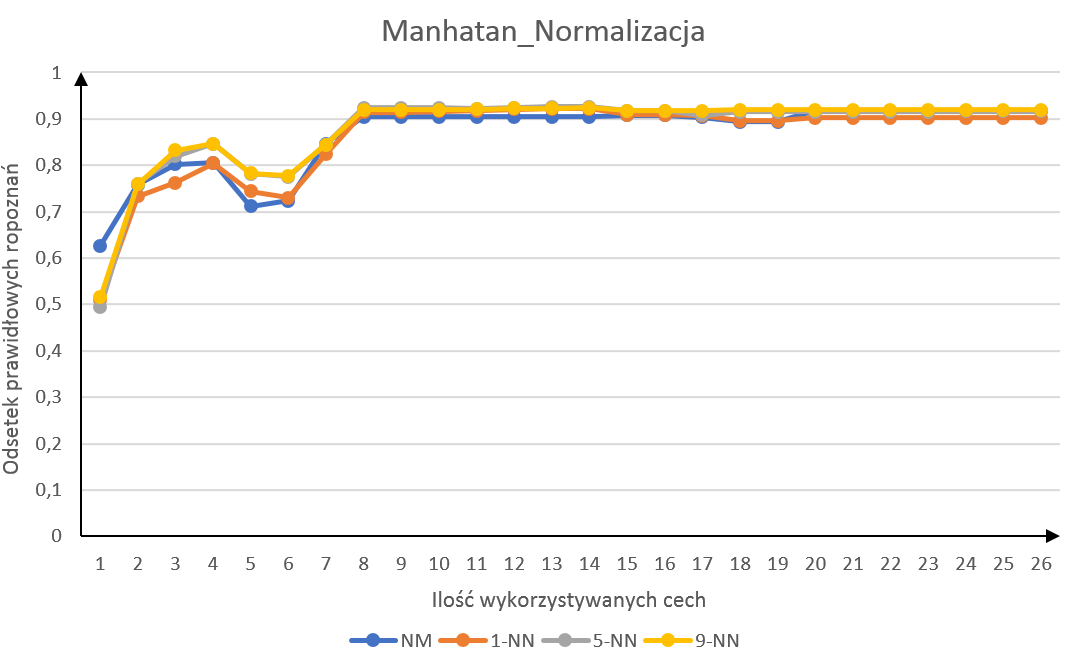
\includegraphics[scale=0.66]{images/algorithms/manhatan_norm.png}
	\caption{Porównanie algorytmów dla metryki odległościowej \textit{Manhatan}}
\end{figure}

\begin{figure}[H]
	\centering
		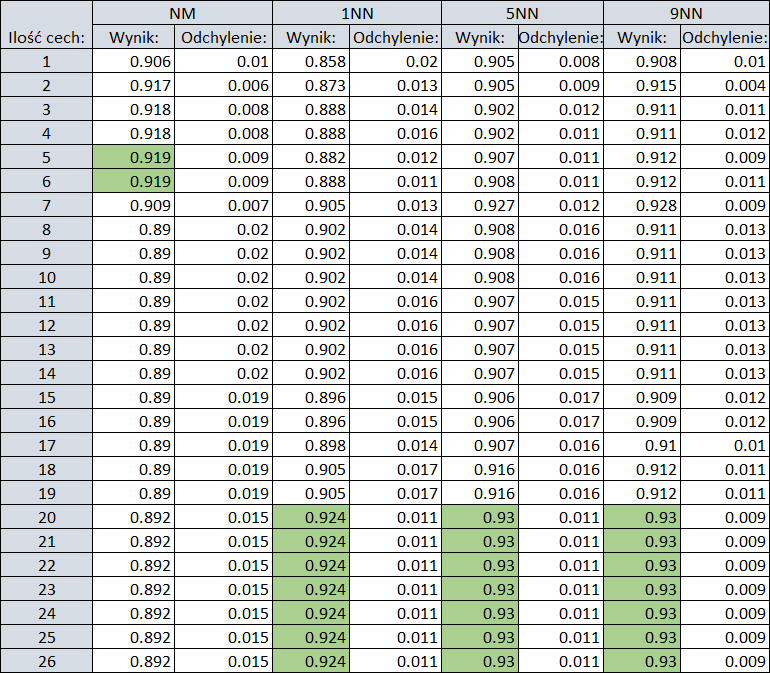
\includegraphics[scale=0.8]{images/algorithms/euklides_beznorm_tab.png}
	\caption{Porównanie algorytmów dla metryki odległościowej \textit{Euklides} bez normalizacji}
\end{figure}
\begin{figure}[H]
	\centering
		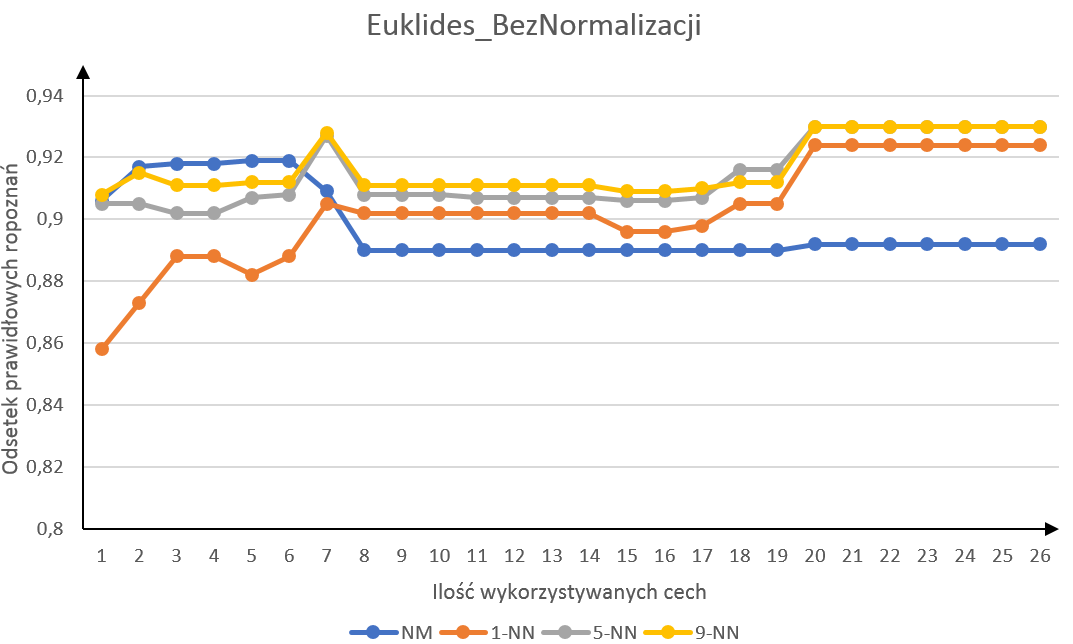
\includegraphics[scale=0.66]{images/algorithms/euklides_beznorm.png}
	\caption{Porównanie algorytmów dla metryki odległościowej \textit{Euklides} bez normalizacji wektorów}
\end{figure}

\begin{figure}[H]
	\centering
		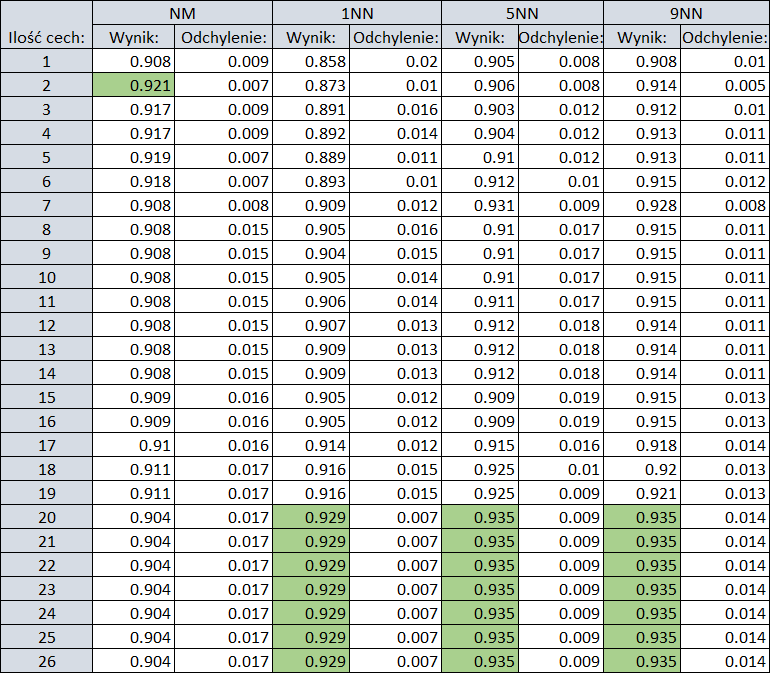
\includegraphics[scale=0.8]{images/algorithms/manhatan_beznorm_tab.png}
	\caption{Porównanie algorytmów dla metryki odległościowej \textit{Manhatan} bez normalizacji}
\end{figure}
\begin{figure}[H]
	\centering
		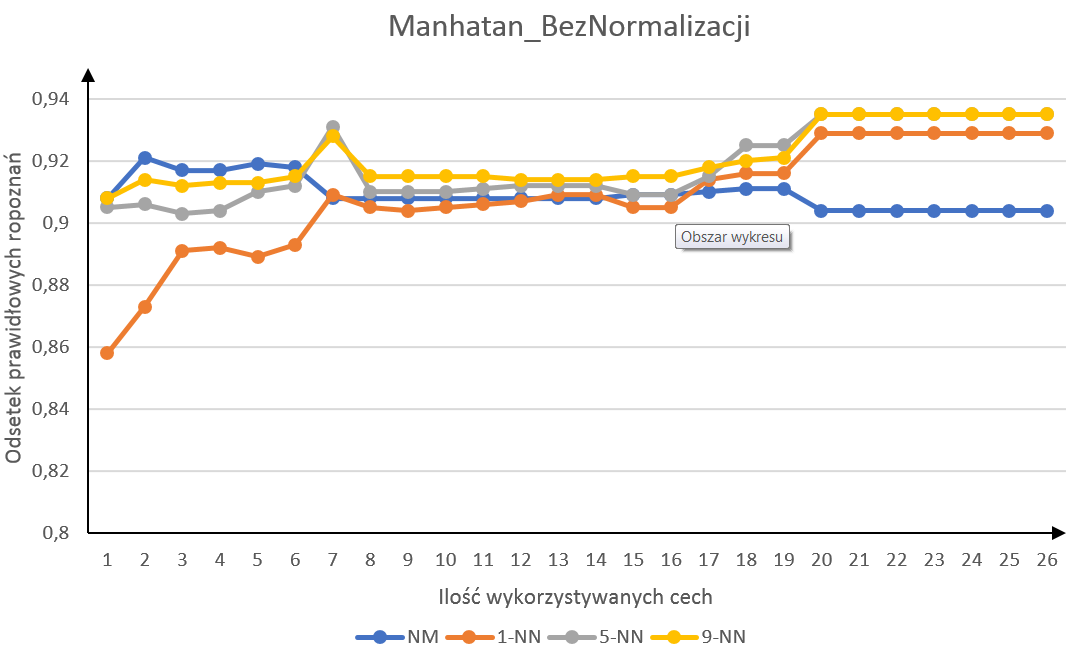
\includegraphics[scale=0.66]{images/algorithms/manhatan_beznorm.png}
	\caption{Porównanie algorytmów dla metryki odległościowej \textit{Manhatan} bez normalizacji}
\end{figure}


% Porównanie metryk odległościowych
\subsection{Porównanie metryk odległościowych}
\begin{figure}[H]
	\centering
		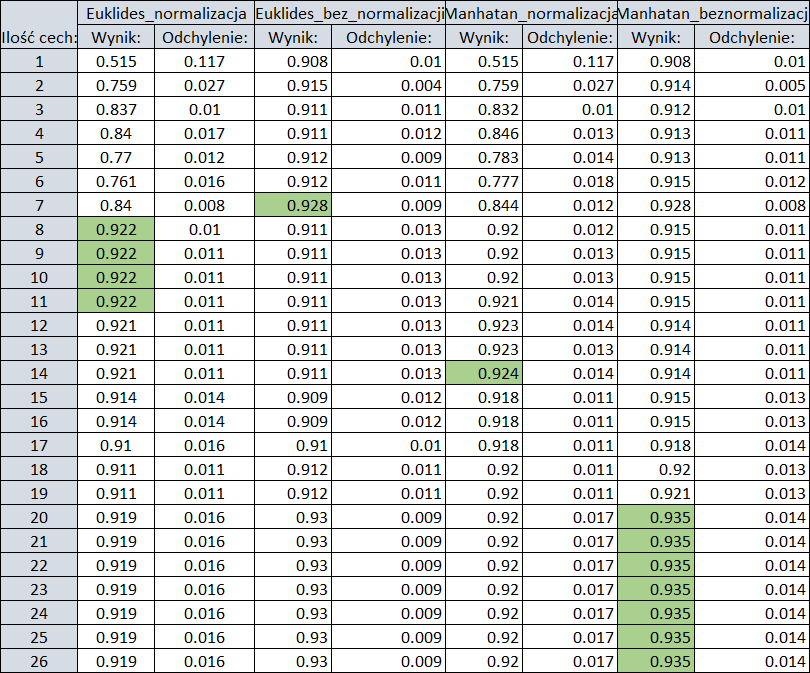
\includegraphics[scale=0.77]{images/distance_metrics/distance_metrics_tab.png}
	\caption{Porównanie metryk odległościowych i reprezentacji wektorów cech}
\end{figure}
\begin{figure}[H]
	\centering
		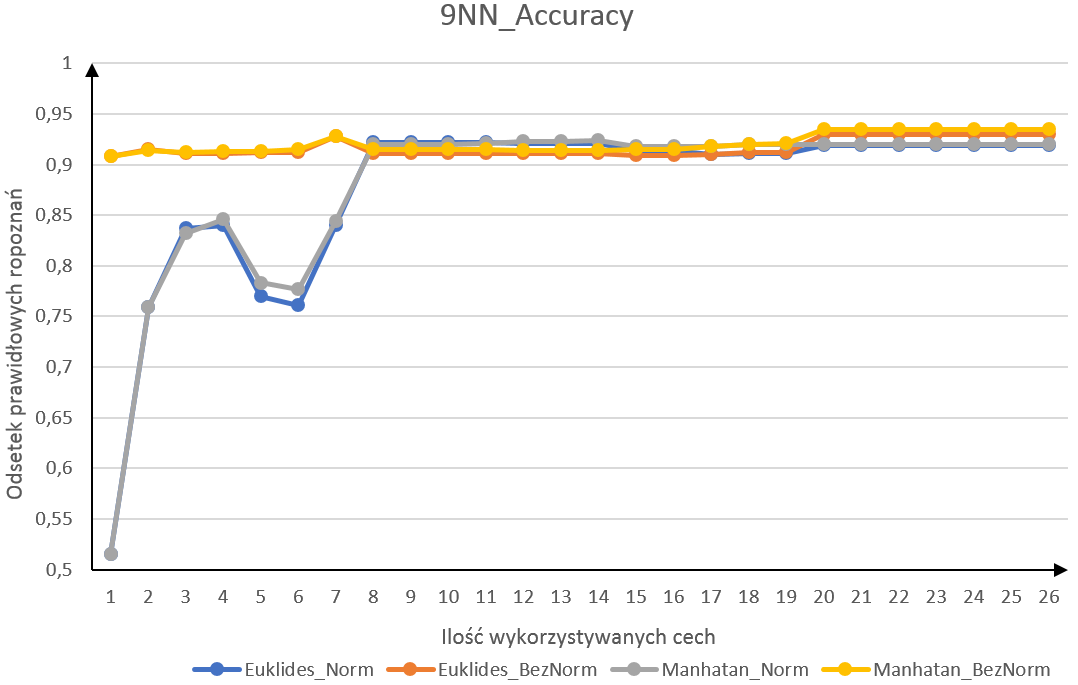
\includegraphics[scale=0.66]{images/distance_metrics/distance_metrics.png}
	\caption{Porównanie metryk odległościowych i reprezentacji wektorów cech}
\end{figure}

%---------------------------------------------------------
%					Część szósta
%---------------------------------------------------------

\section{Dyskusja wyników i wnioski wynikające z badań.}

Porównanie metryk wyszło super, algorytmy śmigały aż miło. Raka diagnozowaliśmy w 90\% a w kolejnych 10\% przepisywaliśmy pacjentkom dodatkowe prywatne badanie cyckuf

\end{document}


